% !TEX root = ../dg.tex

\section{The Exterior Derivative}

We've already seen some calculations of the exterior derivative in local coordinates in \Cref{sec:vector calculus}, but to give a coordinate-free definition of the exterior derivative we need to talk about derivations.

\begin{definition}\label{def:derivation}
	If $V$ is a vector space, an endomorphism $D\from \ext{}(V) \to \ext{}(V)$ of the exterior algebra is
	\begin{itemize}
		\item a \emph{derivation} if $D(u \wedge v) = (Du) \wedge v + u \wedge (Dv)$
		\item an \emph{anti-derivation} if $D(u\wedge v) = (Du) \wedge v + (-1)^k u \wedge (Dv)$ for $u \in \ext{k}(V)$ (notice that this implies that $D(v_1 \wedge \dots \wedge v_m) = \sum_{i=1}^m (-1)^{i-1} v_1 \wedge \dots \wedge v_{i-1} \wedge (D v_i) \wedge v_{i+1} \wedge \dots \wedge v_m$ for any $v_1, \dots , v_m \in V = \ext{1}(V)$)
		\item of \emph{degree} $k$ if $D: \ext{i}(V) \to \ext{i+k}(V)$ for all $i$.
	\end{itemize}
	(This definition extends to any (graded) algebra by substituting the product in the algebra for $\wedge$ in the above.)
\end{definition}

\begin{example}
	We saw on \cpageref{it:linearity of vector field} that tangent vectors can be viewed as (ungraded) derivations on the algebra $\mathcal{D}_p$ of functions which are smooth in a neighborhood of a point $p \in M$. More generally, a vector field $X \in \mathfrak{X}(M)$ is a derivation on the algebra $C^\infty(M)$ because it satisfies the Leibniz rule $X(fg) = (Xf)g + f(Xg)$.
	
	There's no degree in either of these cases because $\mathcal{D}_p$ and $C^\infty(M)$ are ungraded.
\end{example}

\begin{definition}\label{def:exterior derivative}
	The \emph{exterior derivative} $d \from \Omega^\ast(M) \to \Omega^\ast(M)$ is the unique anti-derivation of degree $+1$ so that
	\begin{enumerate}
		\item \label{it:d_0 is differential} For all $f \in C^\infty(M) = \Omega^0(M)$, $df$ is the differential of $f$.
		\item \label{it:d^2=0} $d \circ d = 0$.
	\end{enumerate}
\end{definition}

\begin{proposition}\label{prop:exterior derivative existence and uniqueness}
	There is such a creature and it is unique.
\end{proposition}

The idea is that we kind of know what such an thing should look like in local coordinates around a point $p \in M$: any $k$-form $\omega \in \Omega^k(M)$ can be written in local coordinates as
\[
	\omega_p = \sum_I f_I\, dx_I.
\]
So then define
\begin{equation}\label{eq:exterior derivative local coords}
	(d\omega)_p := \sum_I (df_I) \wedge dx_I.
\end{equation}

\begin{example}\label{ex:1-form in R^3}
	Consider $\omega \in \Omega^1(\R^3)$ given by $\omega = z \, dy + xy \, dz$. Then
	\begin{multline*}
		d\omega = (dz) \wedge dy + (d(xy)) \wedge dz = dz \wedge dy + \left(\frac{\partial (xy)}{\partial x} dx + \frac{\partial (xy)}{\partial y} dy + \frac{\partial (xy)}{\partial z} dz\right) \wedge dz \\
		= dz \wedge dy + y\, dx \wedge dz + x \, dy \wedge dz = y\, dx \wedge dz + (x-1) dy \wedge dz.
	\end{multline*}
\end{example}

I claim that \eqref{eq:exterior derivative local coords} is the only way to get an anti-derivation of degree $+1$ that satisfies \ref{it:d_0 is differential} and \ref{it:d^2=0} in local coordinates. Why? If $d$ satisfies \ref{it:d_0 is differential} and \ref{it:d^2=0}, then $dx_i = d(x_i)$ is the result of applying $d$ to the 0-form $x_i$ (by \ref{it:d_0 is differential}), so $d(dx_i) = (d \circ d)(x_i) = 0$ (by \ref{it:d^2=0}). But then the anti-derivation property implies that
\[
	d(dx_I) = d(dx_{i_1} \wedge \dots \wedge dx_{i_k}) = \sum_{j=1}^k(-1)^{j-1} dx_{i_1} \wedge \dots \wedge dx_{i_{j-1}} \wedge d(dx_{i_j}) \wedge dx_{i_{j+1}} \wedge \dots \wedge dx_{i_k} = 0
\]
since each $d(dx_{i_j}) = 0$. But then, again applying the anti-derivation condition together with linearity,
\[
	(d\omega)_p = d\left(\sum_I f_I\, dx_I\right) = \sum_I \left[ (df_I) \wedge dx_I + f_I\, d(dx_I)\right] = \sum_I (df_I) \wedge dx_I.
\]

\begin{exercise}
	Go back to \Cref{sec:vector calculus} and verify the various exterior derivative calculations we did there.
\end{exercise}

\begin{proof}[Proof of \Cref{prop:exterior derivative existence and uniqueness}]
	Define $d$ in local coordinates as in \eqref{eq:exterior derivative local coords}. Independence of the choice of coordinates will follow from uniqueness, so it remains to show:
	\ifpdf
		\begin{enumerate}[label=(\alph*)]
			\item \label{it:local anti-derivation} This is an anti-derivation.
			\item \label{it:local cocycle} It satisfies the cocycle condition \ref{it:d^2=0}.
			\item \label{it:local uniqueness} Uniqueness.
		\end{enumerate}
		
	\else
		\begin{description}
			\item [(a)\label{it:local anti-derivation}] This is an anti-derivation.
			\item [(b)\label{it:local cocycle}] It satisfies the cocycle condition \ref{it:d^2=0}.
			\item [(c)\label{it:local uniqueness}] Uniqueness.
		\end{description}
	\fi
	
	\ifpdf\ref{it:local anti-derivation} \else (a) \fi and \ifpdf\ref{it:local cocycle} \else (b) \fi are both computations. Here's the computation for \ifpdf\ref{it:local cocycle}\else (b)\fi: If $\omega = \sum_I f_I\, dx_I$ in a neighborhood of $p \in M$, then 
	\[
		d\omega = \sum_I df_I \wedge dx_I = \sum_I \left( \sum_{i=1}^n \frac{\partial f}{\partial x_i} dx_i\right) \wedge dx_I
	\]
	in that same neighborhood, so
	\[
		d(d\omega) = \sum_I \left( \sum_{i=1}^n d\left(\frac{\partial f}{\partial x_i}\right) \wedge dx_i\right) \wedge dx_I = \sum_I \left( \sum_{i=1}^n \left(\sum_{j=1}^n\frac{\partial^2 f}{\partial x_j\partial x_i} dx_j\right) \wedge dx_i\right) \wedge dx_I = 0
	\]
	since $\frac{\partial^2 f}{\partial x_j\partial x_i} = \frac{\partial^2 f}{\partial x_i\partial x_j}$ but $dx_j \wedge dx_i = - dx_i \wedge dx_j$.
	
	Turning to \ifpdf\ref{it:local uniqueness}\else (c)\fi, suppose there exists a degree $+1$ anti-derivation $D\from \Omega^\ast(M) \to \Omega^\ast(M)$ satisfying \ref{it:d_0 is differential} and \ref{it:d^2=0}. In particular, $Df = df$ for all $f \in C^\infty(M) = \Omega^0(M)$. Then
	\[
		D(dx_I) = D(dx_{i_1} \wedge \dots \wedge dx_{i_k}) = \sum_{j=1}^k (-1)^{j-1} dx_{i_1} \wedge \dots \wedge dx_{i_{j-1}} \wedge D(dx_{i_j}) \wedge dx_{i_{j+1}} \wedge \dots \wedge dx_{i_k} = 0
	\]
	since $\displaystyle D(dx_{i_j}) \mathop{=}\limits^{\ref{it:d_0 is differential}} D(Dx_{i_j}) \mathop{=}\limits^{\ref{it:d^2=0}} 0$ by hypothesis.
	
	Therefore, if $\omega = \sum_I f_I dx_I$ in a neighborhood of $p$, by linearity and the anti-derivation condition we have
	\[
		D\omega = \sum_I (Df_I \wedge dx_I + f_I D(dx_I)) = \sum_I Df_I \wedge dx_I \mathop{=}^{\ref{it:d_0 is differential}} \sum_I df_I \wedge dx_I = d\omega
	\]
	in that neighborhood. Since this is true for all $p \in M$, it must be the case that $D\omega = d\omega$.
\end{proof}

Notice that $d$ being degree $+1$ and satisfying the cocycle condition \ref{it:d^2=0} says exactly that we have a diagram
	\begin{center}
	\begin{tikzcd}
		\Omega^0(M) \arrow[r,"d"] & \Omega^1(M) \arrow[r,"d"] &  \dots \arrow[r,"d"] & \Omega^{n-1}(M) \arrow[r,"d"] & \Omega^n(M) 
	\end{tikzcd}
	\end{center}
which is a cochain complex.
	
\begin{definition}\label{def:closed and exact}
	A differential form $\omega \in \Omega^k(M)$ is \emph{closed} if $d\omega = 0$ and it is \emph{exact} if $\omega = d\eta$ for some $\eta \in \Omega^{k-1}(M)$. Notice that, by the cocycle condition \ref{it:d^2=0}, all exact forms are closed.
\end{definition}

\begin{exercise}\label{ex:closed not exact}
	Show that $\omega \in \Omega^1(\R^2 - \{0\})$ given by $\omega = \frac{x\, dy - y \, dx}{x^2 + y^2}$ is closed but not exact. (Using the correspondence between 1-forms and vector fields, this is equivalent to the fact that the vector field $\left(\frac{-y}{x^2 + y^2}, \frac{x}{x^2+y^2}\right)$ is curl-free but not a gradient field.)
\end{exercise}

\section{Pullbacks}
\label{sec:pullbacks}

Suppose we have manifolds $M$ and $N$ and a smooth map $f \from M \to N$. Since we have a change of variables formula for integrals, and differential forms are supposed to be the objects that we can integrate on manifolds, we should expect that $f$ gives a way of turning differential forms on one of $M$ or $N$ into forms on the other. If you think about how the change of variables formula works, you can figure out which direction this is supposed to go, but let's build up to this a bit more slowly.

First of all, recall that if $v \in T_pM$, then $df_p v \in T_{f(p)}N$; that is, $df_p \from T_pM \to T_{f(p)}N$. More precisely, since $v = \alpha'(0)$ for some smooth curve $\alpha$ with $\alpha(0) = p$, we defined $df_pv = (f \circ \alpha)'(0)$. In words, $f$ gives a way of pushing tangent vectors forward using $df$,\footnote{In fact, many books and papers use the notation $f_\ast$ rather than $df$ since this is the standard notation for a pushforward operator.} and we could have guessed this in advance because $v$ is defined in terms of a map into $M$, which can then be composed with $f$ to get a map into $N$. In categorical terms, tangent vectors and vector fields are transformed \emph{covariantly}, meaning that tangent vectors or vector fields get sent in the same direction (from $M$ to $N$) as the original map $f\from M \to N$.

Now let's think about how we could move differential forms around using $f$. At a point, a $k$-form $\omega \in \Omega^k(M)$ corresponds to $\omega_p \in \ext{k}\left(\left(T_pM\right)^\ast\right) \cong \left(\ext{k}\left(T_pM\right)\right)^\ast$, or equivalently an alternating multilinear functional $\left(T_pM\right)^k \to \R$. In other words, unlike a tangent vector which is defined by a map \emph{into} $M$, a differential form corresponds to a map \emph{out of} $\left(T_pM\right)^k$. That means there's really no way to compose $\omega_p \in \ext{k}\left(\left(T_pM\right)^\ast\right)$ with $f$ to get something on $N$.

However, if we start instead with $\eta \in \Omega^k(N)$, then, as above, at a point $q \in N$, $\eta_q$ corresponds to a map $\left(T_qN\right)^k \to \R$, so we \emph{should} be able to precompose with a map $\left(T_pM\right)^k \to \left(T_q N \right)^k$ to get a $k$-form on $M$. More precisely:

\begin{definition}\label{def:pullback}
	If $f \from M \to N$ is smooth and $\eta \in \Omega^k(N)$, then the \emph{pullback} of $\eta$ by $f$ is the form $f^\ast \eta \in \Omega^k(M)$ defined by
	\[
		(f^\ast \eta)_p(v_1, \dots , v_k) := \eta_{f(p)}(df_p v_1, \dots, df_pv_k)
	\]
	for any $v_1, \dots , v_k \in T_pM$.
\end{definition}

Notice, first of all, that this definition makes sense because $df_p\from T_pM \to T_{f(p)}N$, so each $df_p v_i \in T_{f(p)}N$, and hence can be fed into $\eta_{f(p)}$. 

In the paragraph before \Cref{def:pullback} I said we could precompose $\eta$ with a map $\left(T_pM\right)^k \to \left(T_q N \right)^k$, but then didn't write down such a map. What's going on here? The differential $df_p \from T_p M \to T_{f(p)}N$ induces a map $\left(df_p\right)^k \from \left(T_p M\right)^k \to \left(T_{f(p)}N\right)^k$ by just applying $df_p$ separately in each factor. So then another way of stating \Cref{def:pullback} is that 
\[ 
	(f^\ast \eta)_p = \eta_{f(p)} \circ (df_p)^k.
\]

\begin{example}\label{ex:pullbacks of functions are compositions}
	Suppose $g \in \Omega^0(N) = C^\infty(N)$. then 
	\[
		(f^\ast g)_p = g_{f(p)} = g(f(p)) = (g \circ f)(p),
	\]
	recalling that, for a form $\omega$, the notation $\omega_p$ really just means $\omega(p)$.
	
	In other words, $f^\ast g = g \circ f$.
\end{example}

\begin{example}\label{ex:unit circle pullback dx}
	Let $f \from S^1 \to \R^2$ be the inclusion of the unit circle into the plane; i.e., $f(\theta) = (\cos \theta , \sin \theta)$. Let $\omega = dx \in \Omega^1(\R^2)$, which at each point $p \in \R^2$ is computed by $dx\left(a \frac{\partial}{\partial x} + b \frac{\partial}{\partial y}\right) = a$; or, said another way, by taking the dot product of the input tangent vector with the first standard basis vector.
	
	What is $f^\ast \omega = f^\ast dx$? At any point $\theta_0 \in S^1$, we have the local coordinate basis $\left\{ \frac{\partial}{\partial \theta}\right\}$ for $T_{\theta_0}S^1$, so we can completely specify $f^\ast dx$ by determining the value of
	\[
		(f^\ast dx)_{\theta_0}\left( a \frac{\partial}{\partial \theta}\right)
	\]
	for any $a \in \R$. By \Cref{def:pullback},
	\[
		(f^\ast dx)_{\theta_0}\left( a \frac{\partial}{\partial \theta}\right) = (dx)_{f(\theta_0)}\left(df_{\theta_0}\left( a \frac{\partial}{\partial \theta}\right)\right).
	\]
	So first we'll need to compute $df_{\theta_0}\left( a \frac{\partial}{\partial \theta}\right)$. We can write $a \frac{\partial}{\partial \theta} = \alpha'(0)$, where $\alpha(t) = \theta_0 + a t$, so \Cref{def:differential} tells us that
	\begin{multline*}
		df_{\theta_0}\left( a \frac{\partial}{\partial \theta}\right) = (f \circ \alpha)'(0) = \left. \frac{d}{dt} \right|_{t=0} f(\alpha(t)) = \left. \frac{d}{dt} \right|_{t=0} f(\theta_0 + at) = \left. \frac{d}{dt} \right|_{t=0} (\cos(\theta_0 + at), \sin(\theta_0 + at)) \\
		= \left. (-a\sin(\theta_0 + at),a \cos(\theta_0 + at))\right|_{t=0} = (-a \sin(\theta_0), a \cos(\theta_0)) = -a \sin(\theta_0) \frac{\partial}{\partial x} + a \cos(\theta_0) \frac{\partial}{\partial y}
	\end{multline*}
	after switching between tuple notation and local coordinate basis notation. 
	
	Therefore,
	\[
		(f^\ast dx)_{\theta_0}\left( a \frac{\partial}{\partial \theta}\right) = (dx)_{f(\theta_0)}\left(df_{\theta_0}\left( a \frac{\partial}{\partial \theta}\right)\right) = (dx)_{f(\theta_0)}\left(-a \sin(\theta_0) \frac{\partial}{\partial x} + a \cos(\theta_0) \frac{\partial}{\partial y}\right) = -a \sin(\theta_0).
	\]
	
	In other words,
	\[
		(f^\ast dx)_{\theta_0} = -\sin\theta_0 (d\theta)_{\theta_0}
	\]
	or, by slight abuse of notation,
	\[
		f^\ast dx = -\sin \theta \, d\theta.
	\]
	Recalling that $\theta \in S^1$ maps to the point $(\cos \theta, \sin \theta)$, we can see that $\sin \theta$ is the $y$-coordinate, so this could also be written as
	\[
		f^\ast dx = -y \, d\theta.
	\]
	Geometrically, this makes sense: at the point $(x,y) = (\cos \theta, \sin \theta)$ this form is dual to the tangent vector $-y \frac{\partial}{\partial \theta}$, which at each point is just the orthogonal projection of the first standard basis vector $\frac{\partial}{\partial x}$ onto the tangent space to the circle, and of course $\frac{\partial}{\partial x}$ is the tangent vector to $(x,y) \in \R^2$ dual to $dx$. See \Cref{fig:pullback dx}.
	
	\begin{figure}[htbp]
		\centering
			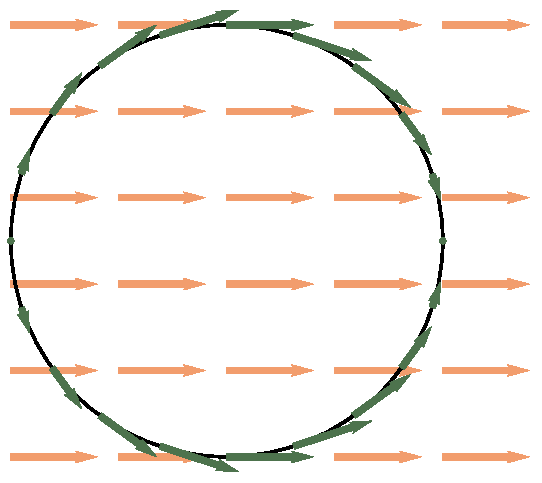
\includegraphics[height=2in]{pullbackdx}
		\caption{The vector field $\frac{\partial}{\partial x}$ (dual to $dx$) on $\R^2$ is shown in orange, and the vector field $-y \frac{\partial}{\partial \theta}$ (dual to $-y\, d\theta = f^\ast dx$) on the circle is shown in green.}
		\alttext{A figure with a white background showing a black circle, a collection of thick orange arrows all of the same length and all pointing to the right, and a collection of thick green arrows of different lengths tangent to various points on the circle.}
		\label{fig:pullback dx}
	\end{figure}
\end{example}

One nice thing about pullbacks is that they commute with the exterior derivative:

\begin{proposition}\label{prop:pullbacks commute with exterior derivative}
	For $f \from M \to N$ smooth and $\omega \in \Omega^k(N)$,
	\[
		d(f^\ast \omega) = f^\ast d\omega.
	\]
\end{proposition}

Before proving this, let's see it in an example:

\begin{example}
	Continuing \Cref{ex:1-form in R^3}, recall that $\omega = z \, dy + xy \, dz$ and we computed 
	\[
		d\omega = y\, dx \wedge dz + (x-1) dy \wedge dz.
	\]
	
	Now, consider the map $f \from \R^2 \to \R^3$ given by $f(u,v) = (u^2, u, uv)$. For $p = (u_0, v_0) \in \R^2$ and $w = a \frac{\partial}{\partial u} + b \frac{\partial }{\partial v} \in T_p\R^2$ for $i=1,2$, we can write $w = \alpha_i'(0)$ where $\alpha_i(t) = p + tw = (u_0 , v_0) + t(a,b)$, so 
	\begin{multline*}
		df_p(w) = (f \circ \alpha_i)'(0) = \left. \frac{d}{dt}\right|_{t=0} ((u_0 + ta)^2, u_0 + ta, (u_0 + ta)(v_0 + tb)) \\
		= (2au_0, a, av_0 + bu_0) = 2au_0 \frac{\partial}{\partial x} + a \frac{\partial}{\partial y} + (av_0 + bu_0) \frac{\partial}{\partial z},
	\end{multline*}
	where I'm going back and forth between tuple notation (in $\R^3$ with the standard basis) and local coordinate basis notation (on $T_{f(p)} \R^3$ with the local coordinate basis [which of course is the same as the standard basis]). 
	
	Therefore,
	\begin{multline*}
		(f^\ast \omega)_p(w) = \omega_{f(p)}(df_p(w)) = \left(\vphantom{x^2} u_0v_0 \, dy + u_0^3 \, dz\right)\left(2au_0 \frac{\partial}{\partial x} + a \frac{\partial}{\partial y} + (av_0 + bu_0) \frac{\partial}{\partial z}\right) \\
		= a u_0 v_0(1+u_0^2) + b u_0^4.
	\end{multline*}
	Since this is what the linear functional $(f^\ast \omega)_{(u_0,v_0)}$ does to the tangent vector $w=a \frac{\partial}{\partial u} + b \frac{\partial }{\partial v}$, we see that $(f^\ast \omega)_{(u_0,v_0)} = u_0 v_0(1+u_0^2) du + u_0^4\, dv$ or, now thinking globally,
	\[
		f^\ast \omega = u v(1+u^2) du + u^4 dv.
	\]
	Hence,
	\begin{align*}
		d(f^\ast \omega) & = \left(d\left( u v(1+u^2) \right)\right) \wedge du + \left(d\left(u^4 \right)\right)\wedge dv \\
		 & = \left( \frac{\partial}{\partial u}\left( u v(1+u^2) \right) du + \frac{\partial}{\partial v}\left( u v(1+u^2) \right) dv\right) \wedge du + \left( \frac{\partial}{\partial u}\left(u^4\right) du + \frac{\partial}{\partial v}\left(u^4\right)dv \right) \wedge dv \\
		 & = u(1+u^2) dv \wedge du + 4u^3 du \wedge dv \\
		 & = (3u^3-u) du \wedge dv.
	\end{align*}
	
	On the other hand,
	\begin{align*}
		(f^\ast d\omega)_{p}\left(\frac{\partial}{\partial u}, \frac{\partial}{\partial v}\right) & = (d\omega)_{f(p)} \left(df_{p}\left(\frac{\partial}{\partial u}\right), df_p\left(\frac{\partial}{\partial v}\right)\right) \\
		 & = \left(\vphantom{x^2}u_0 dx \wedge dz + (u_0^2-1) dy \wedge dz\right)\left(2u_0 \frac{\partial}{\partial x} + \frac{\partial}{\partial y} + v_0\frac{\partial}{\partial z}, u_0\frac{\partial}{\partial z}\right) \\
		 & = 3u_0^3 -u_0.
	\end{align*}
	Notice that $(3u_0^3 -u_0)du \wedge dv $ would produce the same output for this (or any other) input, so $(f^\ast d\omega)_{(u_0,v_0)}= (3u_0^3 -u_0)du \wedge dv$. In other words (now thinking globally)
	\[
		f^\ast d\omega = (3u^3-u)du \wedge dv = d(f^\ast \omega),
	\]
	as predicted by \Cref{prop:pullbacks commute with exterior derivative}.
\end{example}

\begin{proof}[Proof of \Cref{prop:pullbacks commute with exterior derivative}]
	 Let $p \in M$. If $\omega = g\in \Omega^0(N) = C^\infty(N)$, then $f^\ast g = g \circ f$, so $d(f^\ast g ) = d(g \circ f)$. On the other hand, for any $v \in T_pM$, 
	 \[
	 	(f^\ast dg)_pv = dg_{f(p)}(df_p v) = d(g \circ f)_p(v) = d(f^\ast g)_p(v),
	 \]
	 where we used \Cref{def:pullback} for the first equality, the Chain Rule for the second, and \Cref{ex:pullbacks of functions are compositions} for the third. This completes the proof in the $k=0$ case.
	 
	 Now, suppose $k > 0$ and that $x_1, \dots , x_n$ are local coordinates in a neighborhood of $f(p) \in N$, meaning that $\omega \in \Omega^k(N)$ has the form $\omega_{f(p)} = \sum_I g_I dx_I$ at $f(p)$, so that
	 \[
	 	(d\omega)_{f(p)} = \sum_I dg_I \wedge dx_I.
	 \]
	 But then
	 \[
	 	(f^\ast d\omega)_p = \sum_I (f^\ast dg_I) \wedge (f^\ast dx_I) = \sum_I d(g_I \circ f) \wedge f^\ast dx_{i_1} \wedge \dots \wedge f^\ast dx_{i_k} = \sum_I d(g_I \circ f) \wedge d(x_{i_1} \circ f) \wedge \dots \wedge d(x_{i_k} \circ f),
	 \]
	 where we've repeatedly used both the $k=0$ case and the fact that $f^\ast(\alpha \wedge \beta) = (f^\ast \alpha) \wedge (f^\ast \beta)$ (which follows from HW \#2, Problem 1).
	 
	 On the other hand,
	 \[
	 	(f^\ast\omega)_p = \sum_I (g_I \circ f) f^\ast dx_I = \sum_I (g_I \circ f) f^\ast dx_{i_1} \wedge \dots \wedge f^\ast dx_{i_k} = \sum_I (g_I \circ f) d (x_{i_1} \circ f) \wedge \dots \wedge d(x_{i_k} \circ f),
	 \]
	 so
	 \[
	 	(df^\ast \omega)_p = \sum_I d(g_I \circ f) \wedge d (x_{i_1} \circ f) \wedge \dots \wedge d(x_{i_k} \circ f) = (f^\ast d\omega)_p,
	 \]
	 and we conclude that the proposition is also true for $k>0$.
\end{proof}